\begin{activity}{Thermal Diffusivity, Thermal Length, and Timescales}

\section*{Purpose}
To understand transient heat flow in terms of:
\begin{itemize}
  \item how far thermal signals propagate in a given time,
  \item how long it takes thermal changes to affect a given depth,
  \item and how the \emph{thermal length scale} controls signal shape and timing.
\end{itemize}

\section*{Learning Outcomes}

By the end of this activity, you should be able to:
\begin{itemize}
  \item Define thermal diffusivity and explain which material properties control it.
  \item Use the thermal length scale $\ell_T = 2\sqrt{\kappa t}$ to estimate how far a thermal signal has propagated or how long it takes to reach a given depth.
  \item Interpret the error function solution and identify where temperature changes are largest.
  \item Compare thermal diffusion timescales for different materials and connect these to real geological processes, including how long a thermal event at a given crustal or lithospheric depth takes to be felt elsewhere.
\end{itemize}

\ntextbox{Thermal Diffusion: Solution and Scaling}{
\textbf{Half-Space Solution}

For instantaneous heating or cooling at a boundary, the temperature evolution is given by the error function solution:
\[
T(z,t) = T_s + (T_b - T_s)\,\erf \left(\frac{z}{2\sqrt{\kappa t}}\right).
\]

\emph{Important:} the argument of the error function,
\[
\eta = \frac{z}{2\sqrt{\kappa t}},
\]
controls the \emph{shape and timing} of the thermal signal: the temperature change is largest where $\eta$ is small and becomes negligible once $\eta$ is of order 1. That crossover, $\eta\sim1$, is what defines the characteristic depth below.

\begin{center}
    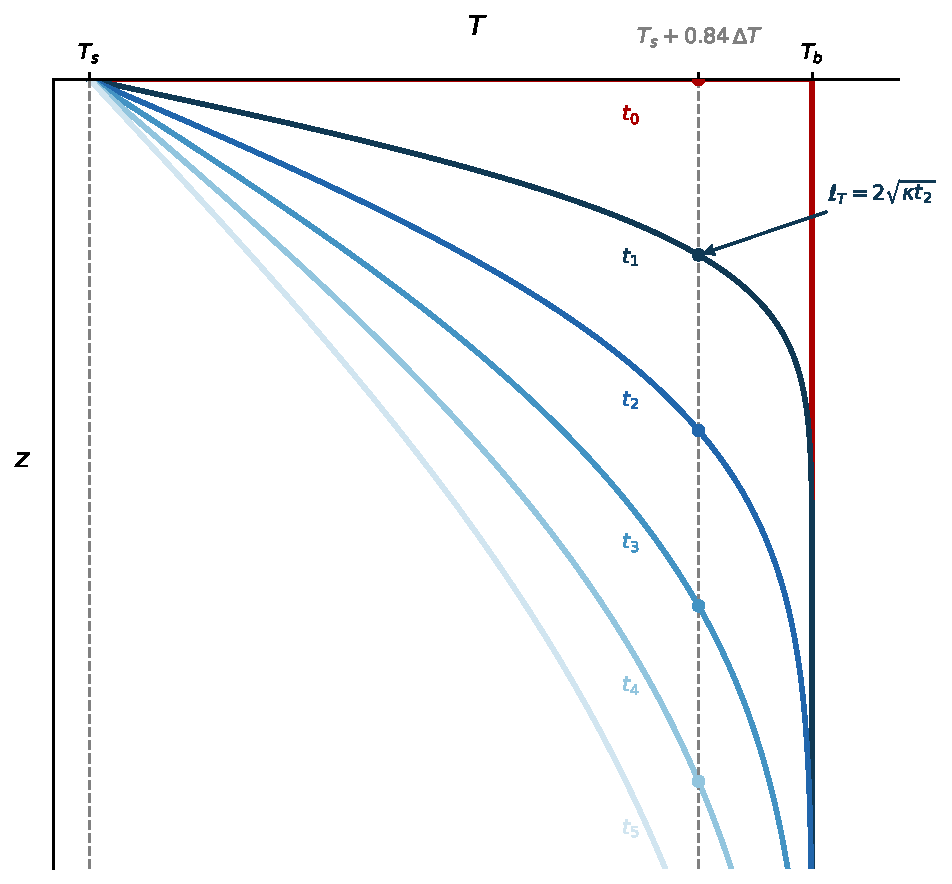
\includegraphics[width=0.6\textwidth]{figures/halfspace_cooling.pdf}
    \captionof{figure}{Half-space cooling at several time intervals. Each curve reaches $T_s+0.84\,\Delta T$ (dashed line) at its own thermal length $\ell_T=2\sqrt{\kappa t}$ -- the same fractional temperature change, at a depth that grows with time.}
    \label{fig:halfspace}
\end{center}

\medskip
\textbf{Thermal Length and Characteristic Time}

For diffusion-dominated heat transfer, the characteristic depth over which temperature changes propagate scales as
\[
z \sim 2 \sqrt{\kappa t}.
\]

This thermal length sets both:
\begin{itemize}
  \item the depth to which temperature changes have propagated after time $t$,
  \item the timescale required for a thermal perturbation at depth to influence shallower levels.
\end{itemize}

\medskip
\textbf{Thermal Diffusivity}

Thermal diffusivity is defined as
\[
\kappa = \frac{k}{\rho C_p},
\]
where $k$ is thermal conductivity, $\rho$ is density, and $C_p$ is specific heat.

Thermal conductivity and diffusivity vary with temperature, porosity, mineralogy, fluid content, and fabric. While not simple, there are some typical ranges that one can expect depending on the geologic material (Table~\ref{tab:diffusivity}).

\begin{center}
    \captionof{table}{Representative ranges for thermal conductivity and diffusivity of geologic materials.  Values are rounded for scaling arguments rather than precise modeling.}
    \label{tab:diffusivity}
    \begin{tabular}{lccc}
        \toprule
        \textbf{Material} &
        \textbf{Thermal Conductivity $k$} &
        \textbf{Thermal Diffusivity $\kappa$} &
        \textbf{Thermal Diffusivity $\kappa$} \\
        &
        \textbf{(W m$^{-1}$ K$^{-1}$)} &
        \textbf{(m$^2$ s$^{-1}$)} &
        \textbf{(km$^2$ My$^{-1}$)} \\
        \midrule
        Ice (glacial / ice sheet average) & 1.6--2.0 & $(0.7$--$0.9)\times10^{-6}$ & 22--28 \\
        Clay-rich sediments               & 0.6--1.5 & $(0.2$--$0.5)\times10^{-6}$ & 6--16  \\
        Granite                           & 2.5--3.5 & $(0.8$--$1.2)\times10^{-6}$ & 25--38 \\
        Basalt / Gabbro                   & 1.7--2.2 & $(0.6$--$1.0)\times10^{-6}$ & 19--32 \\
        Peridotite (upper mantle)         & 3.3--4.5 & $(1.0$--$1.5)\times10^{-6}$ & 32--47 \\
        \bottomrule
    \end{tabular}
\end{center}
}{core}

\section*{Tasks}
\begin{questions}

\question{Rock vs.\ Ice}

Using the diffusivity table, compute the thermal length $\ell_T=2\sqrt{\kappa t}$ for rock (use granite, $\kappa\approx30$~km$^2$/My) and for ice ($\kappa\approx25$~km$^2$/My) at each timescale below. The first row is worked for you.

\begin{center}
\begin{tabular}{cccc}
\toprule
$t$ (yr) & $t$ (My) & $\ell_T$, rock (km) & $\ell_T$, ice (km) \\
\midrule
$10^3$ & $10^{-3}$ & 0.35 & 0.32 \\
$10^5$ &           &      & \\
$10^7$ &           &      & \\
\bottomrule
\end{tabular}
\end{center}

\begin{enumerate}[label=(\alph*)]
  \item Describe how the depth of thermal influence differs between rock and ice at each timescale.
  \answerbox[2.5cm]

  \item Explain why borehole paleothermometry in rock requires much greater depths to recover long-term climate signals than ice-core records -- is it mainly a difference in $\kappa$, or something else?
  \answerbox[2.5cm]
\end{enumerate}

\question{Distance Given Time}

\begin{enumerate}[label=(\alph*)]
  \item For a fixed time $t$, describe how temperature varies with depth $z$ as the value of $\eta$ increases.
  \answerbox[2cm]

  \item Explain why temperature changes are largest for $\eta \ll 1$ and become negligible for $\eta \gg 1$.
  \answerbox[2cm]

  \item Using Figure~\ref{fig:halfspace}, how does the depth at which 84\% of $\Delta T$ has been reached change between $t_1$, $t_2$, and $t_3$? Does it scale the way you'd expect from $\ell_T=2\sqrt{\kappa t}$?
  \answerbox[2cm]
\end{enumerate}

\question{Time Given Distance: How Long Does a Thermal Event Take to Be Felt?}

Rearranging the thermal length relation,
\[
t \sim \frac{z^2}{4\kappa},
\]
gives the timescale for heat to travel a distance $z$. Using $\kappa\approx30$~km$^2$/My (representative crust/mantle value), complete the table below. The first row is worked for you.

\begin{center}
\begin{tabular}{lcc}
\toprule
Depth & $z$ (km) & $t$ (My) \\
\midrule
Mid-lower crust & 20  & 3.3 \\
Moho            & 35  & \\
LAB             & 100 & \\
\bottomrule
\end{tabular}
\end{center}

\begin{enumerate}[label=(\alph*)]
  \item Consider a plume impinging on the base of the lithosphere. Using your table, roughly how long would it take before this thermal perturbation could influence surface temperatures?
  \answerbox[2cm]

  \item Following delamination of a dense crustal root, heat is supplied from below. Using your table, explain why crustal heating is delayed rather than instantaneous -- and delayed by roughly how long?
  \answerbox[2.5cm]
\end{enumerate}

\question{Interpreting ``Arrival'' of Heat}

\begin{enumerate}[label=(\alph*)]
  \item Does heat arrive at a specific time, or does it diffuse gradually? Use the error function shape in Figure~\ref{fig:halfspace} to justify your answer.
  \answerbox[2cm]

  \item For $\eta \approx 1$, what fraction of the total temperature change has occurred? What does this imply about defining a single thermal ``response time''?
  \answerbox[2cm]

  \item Discuss why the concept of a sharp thermal front is inappropriate for diffusion-dominated heat transport.
  \answerbox[2cm]
\end{enumerate}

\end{questions}

\section*{Geological Interpretation}

\begin{itemize}
  \item Thick lithosphere acts as a strong thermal filter, delaying surface response to basal heating.
  \item Thermal signals generated at depth are attenuated and spread out in time as they propagate upward.
  \item The thermal length scale controls which geological processes can be observed at the surface, and on what timescales.
\end{itemize}

\section*{Key Ideas}

\textbf{Diffusion has a characteristic relationship between time and space.} In diffusion problems, time and distance are interchangeable through the thermal length $\ell_T = 2\sqrt{\kappa t}$. A thermal perturbation at the Moho takes millions of years to be felt at the surface; one at the base of the lithosphere takes tens of millions -- diffusion is slow enough that most crustal thermal events are, for practical purposes, invisible at the surface on human timescales.

\begin{center}
\begin{tikzpicture}
  
\end{tikzpicture}
\end{center}

\textbf{Depth and time trade off along straight lines, not a single front.} Each value of $\eta = z/(2\sqrt{\kappa t})$ traces a straight line through the origin in a plot of $z$ against $\sqrt{\kappa t}$, since $z = 2\eta\sqrt{\kappa t}$. A small $\eta$ (strongly affected) and a large $\eta$ (essentially unaffected) bound a widening wedge rather than a sharp edge, so ``has heat arrived here yet?'' only has an answer once you specify how much temperature change counts as arrival.

\begin{figure}[h]
\centering
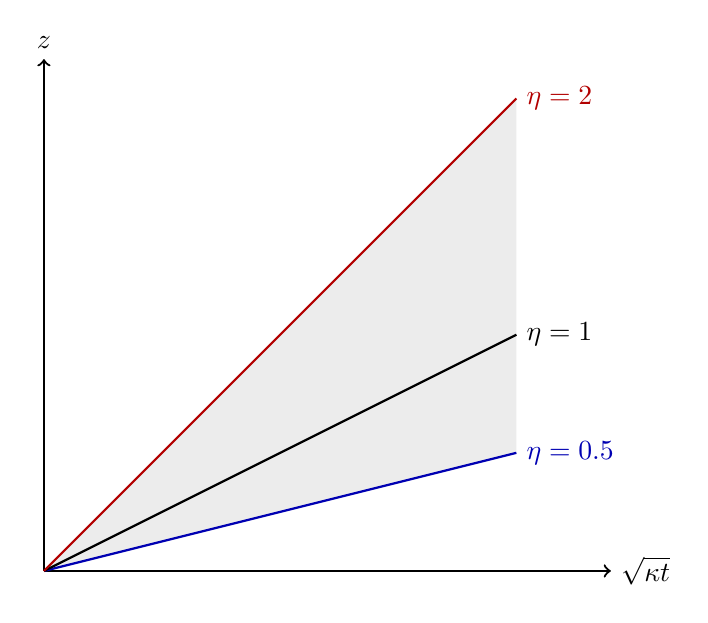
\begin{tikzpicture}[xscale=2,yscale=0.5]
    \draw[->,thick] (0,0) -- (3.6,0) node[right] {$\sqrt{\kappa t}$};
    \draw[->,thick] (0,0) -- (0,13) node[above] {$z$};

    \fill[gray!15] (0,0) -- (3,3) -- (3,12) -- cycle;

    \draw[thick,blue!70!black] (0,0) -- (3,3) node[right] {$\eta=0.5$};
    \draw[thick,black]         (0,0) -- (3,6) node[right] {$\eta=1$};
    \draw[thick,red!70!black]  (0,0) -- (3,12) node[right] {$\eta=2$};
\end{tikzpicture}
\caption{Depth $z$ versus $\sqrt{\kappa t}$ at fixed $\eta = z/(2\sqrt{\kappa t})$. Each $\eta$ traces a straight line of slope $2\eta$; the shaded wedge between $\eta=0.5$ and $\eta=2$ spans the range over which the thermal response fades from strong to negligible, rather than switching off at a single depth.}
\label{fig:eta_lines}
\end{figure}

\end{activity}
